% L12a: the five parts of an agent-based model as one loop (November 5, 2026; replaces the
% lecture's five bullets at the instructor's request). Information goes to the agents, each agent's
% decision rule turns it into an action, the actions add up to the aggregate, and the aggregate
% feeds back into what the agents see next. Same palette as the two model schematics: orange marks
% the aggregate and the feedback.
\documentclass[tikz,border=6pt]{standalone}
% Shared style for the L12a schematics (November 5, 2026), \input by each Fig-L12a-*.tex.
% Same fonts, ink, and accent colors as the L11a/L11b profit diagrams. The notebook SVG
% carries a dark palette added by theme_svg.py; every color here must be mapped there.
\usepackage[no-math]{fontspec}
\IfFontExistsTF{Arial}{\setsansfont{Arial}}{\setsansfont{TeX Gyre Heros}}
\renewcommand{\familydefault}{\sfdefault}
\usepackage{amsmath,amssymb}
\usepackage{array}
\usetikzlibrary{arrows.meta,calc,positioning,decorations.pathreplacing,shapes.geometric}

\definecolor{vnink}{HTML}{202124}
\definecolor{gdblue}{HTML}{0091FF}
\definecolor{gdred}{HTML}{E02020}
\definecolor{gdgray}{HTML}{6D7278}
\definecolor{saorange}{HTML}{F08C00}
\definecolor{boxfill}{HTML}{F1F3F4}
\definecolor{orangefill}{HTML}{FFE8C7}
\definecolor{bluefill}{HTML}{E5F3FF}
\definecolor{redfill}{HTML}{FDE8E8}
\definecolor{gridgray}{HTML}{E3E5E8}

\tikzset{
  every picture/.append style={x=1cm, y=1cm, font=\sffamily\small, text=vnink},
  flow/.style={draw=vnink, line width=0.9pt, -{Latex[length=2.4mm, width=1.7mm]}},
  feedback/.style={draw=saorange, line width=1.2pt, -{Latex[length=2.6mm, width=1.9mm]}, rounded corners=6pt},
  scorefeed/.style={draw=gdblue, line width=1.2pt, dash pattern=on 5pt off 3pt, -{Latex[length=2.6mm, width=1.9mm]}, rounded corners=6pt},
  agent/.style={draw=vnink, fill=boxfill, line width=0.8pt, rounded corners=3pt, minimum width=1.75cm, minimum height=1.05cm, align=center},
  token/.style={draw=vnink, fill=white, line width=0.7pt, minimum width=0.72cm, minimum height=0.6cm, inner sep=1pt},
  oldtoken/.style={text=gdgray, minimum width=0.72cm, minimum height=0.6cm, inner sep=1pt},
  action/.style={circle, draw=vnink, fill=white, line width=0.8pt, minimum size=0.78cm, inner sep=0pt},
  minority/.style={draw=saorange, fill=saorange, text=white, line width=0.8pt, minimum width=0.8cm, minimum height=0.66cm, font=\sffamily\small\bfseries},
  sumbox/.style={draw=vnink, fill=boxfill, line width=0.8pt, rounded corners=3pt, inner sep=5pt, align=center},
  note/.style={text=gdgray, font=\sffamily\footnotesize, align=center},
  paneltitle/.style={anchor=west, font=\sffamily\normalsize},
  state/.style={circle, draw=vnink, fill=white, line width=1.0pt, minimum size=1.25cm, inner sep=0pt, font=\sffamily\normalsize},
}


\begin{document}
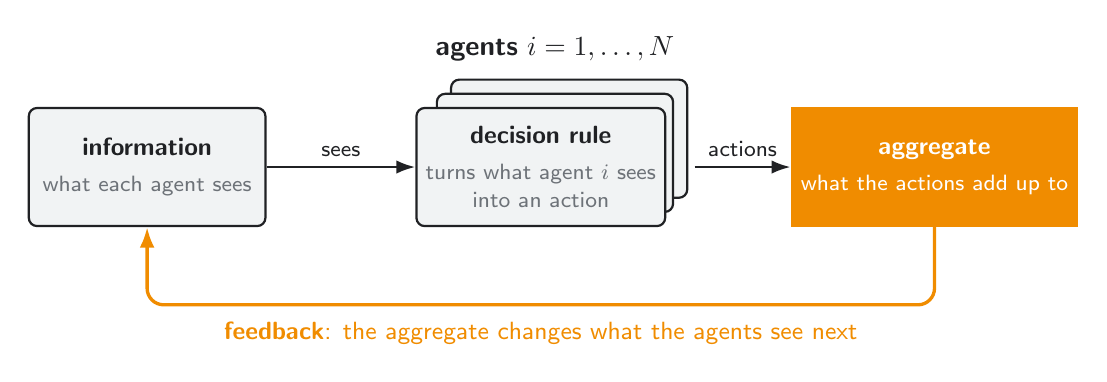
\begin{tikzpicture}
  % information
  \node[sumbox, minimum width=3.0cm, minimum height=1.5cm] (info) at (0, 0) {\textbf{information}\\[2pt]{\footnotesize\color{gdgray}what each agent sees}};

  % agents: a stack of cards, each with its own decision rule
  \foreach \k/\dx in {3/0.36, 2/0.18} {
    \node[agent, minimum width=3.0cm, minimum height=1.5cm] at (5.0+\dx, 0.0+\dx) {};
  }
  \node[agent, minimum width=3.0cm, minimum height=1.5cm] (agents) at (5.0, 0) {\textbf{decision rule}\\[2pt]{\footnotesize\color{gdgray}turns what agent $i$ sees}\\[-1pt]{\footnotesize\color{gdgray}into an action}};
  \node[anchor=south, font=\sffamily\normalsize] at (5.18, 1.22) {\textbf{agents} $i=1,\dots,N$};

  % aggregate
  \node[minority, minimum width=3.0cm, minimum height=1.5cm, align=center, font=\sffamily\small] (agg) at (10.0, 0) {\textbf{aggregate}\\[2pt]{\footnotesize what the actions add up to}};

  % flow
  \draw[flow] (info.east) -- (agents.west) node[midway, above, font=\sffamily\footnotesize] {sees};
  \draw[flow] ($(agents.east)+(0.36,0)$) -- (agg.west) node[midway, above, font=\sffamily\footnotesize] {actions};

  % feedback
  \draw[feedback] (agg.south) -- (10.0, -1.75) -- (0, -1.75) -- (info.south);
  \node[anchor=north, text=saorange, font=\sffamily\small] at (5.0, -1.85) {\textbf{feedback}: the aggregate changes what the agents see next};
\end{tikzpicture}
\end{document}
